	To evaluate the performance of our algorithms we established a base line that predicts random labels for sentiment and kind, and for when we predicted everything as ``current'' time. The accuracy values for assigning these labels to the test set is shown below:

\begin{center}
When accuracy = 77.6\%, Sentiment accuracy  = 16.5\%, Kind Accuracy = 30.3\%
\end{center}

	We will compare these baseline accuracies to the accuracies of our learning algorithms to measure their performance. Note: the ``when'' baseline was determined by always guessing that the time frame was ``current time''. This means that 77.6\% of our tweets are about the current weather. 

\subsubsection{Decision Trees}
	Decision trees performed relatively well and produced reasonable accuracies for the three different categories. The graph below shows the accuracy values against varying tree height for the ``when'' and ``sentiment'' labels. Based on the graph, there does not appear to be dramatic changes in accuracy with varying tree height, however we can see the overfitting and underfitting portions of the graph. 

%DECISION TREE ACCURACY VS TREE DEPTH
\begin{figure}[H]
\noindent\makebox[\textwidth][c]{%
\minipage{0.65\textwidth}%
  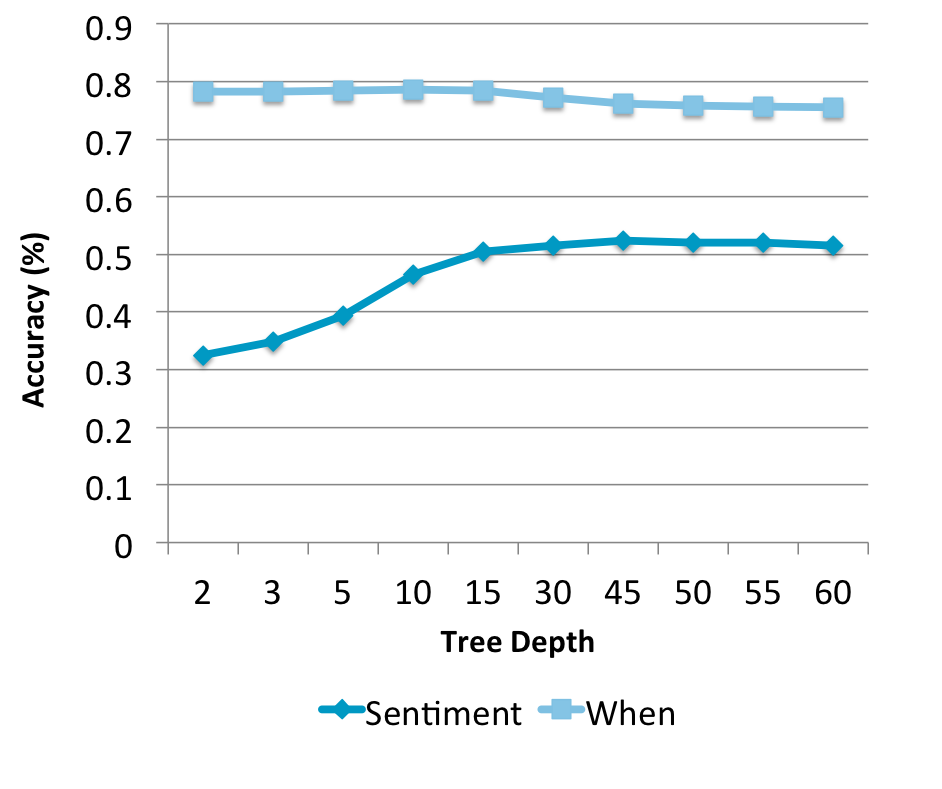
\includegraphics[width=\linewidth]{results/decision}
  \caption{Accuracy vs. Tree Depth}\label{fig:decision}
\endminipage}
\end{figure}

	The optimal height for the ``when'' label is 10 while the optimal height for the ``sentiment'' label is 45. This implies that the decision tree requires much more information to predict the sentiment of a tweet as oppose to the time frame of a tweet. Also, the decision tree was able to predict the ``when'' label of a tweet with a much higher accuracy of 78.6\%, while only a 52.9\% accuracy for the ``sentiment'' label. However, the baseline for the ``when'' label was 76.7\%, so the accuracy for the decision tree is not much higher. This indicates that the decision tree was not very effective in classifying the time frame of a tweet. Since, the baseline for ``when'' is already so high, it is hard to create a classifier that performs significantly better.   

            The decision tree models performed very well for the weather ``kind'' label. As mentioned earlier, multiple trees were used to classify either ``positive'' or ``negative'' for each of the different kinds of weather. All fifteen decision trees with a height of 30 produced accuracies above 95\%. This seems fairly high, but it is plausible because the presences of key words is the strongest indicator of the ``kind'' of weather in a tweet. For example, the word at the root node for each the decision trees has been the type of weather itself. For example the root node for the decision tree classifying whether a tweet is about cold weather is the word ``cold.'' 

	Another reason for the high accuracies values may be due to the change from confidence scores to binary values. We stated earlier that confidence scores above 0.7 are considered positive and confidence scores below 0.3 are considered negative. This means that only tweets that are clearly about a certain type of weather will be classified as either positive or negative. Thus, these are the tweets that explicitly say what the weather is by using descriptive words. However, by doing this we may be ignoring tweets where the weather can be inferred from the meaning behind the texts. These are the tweets that the decision trees may not perform as well on because it cannot rely solely on the presence of key words. Thus, the accuracy values may be lower if we changed the threshold on the confidence scores. 

\subsubsection{Support Vector Machines}

The input dataset from Kaggle was converted into the Svmlight format, which included obtaining the ``best features'' that the Naïve Bayes algorithm produced as the ``important bag of words'', and creating the svmlight format from those particular word counts. We used Professor Joachims’s svmlight module executable to learn classifying models for each of the 24 labels, with varying c-values (to indicate the ``slack'' allowed for the classifier). For each label, the best c-values (that produced the highest accuracy on the validation set) were used to prevent over-fitting in the final classifiers. These classifiers were inherently binary, and gave the geometric margin of a validation tweet from the separator. This geometric margin (normalized) was used to determine best the sentiment and when labels (by taking the max), and the best kind labels (those that were >= 0.7).
 
 
The SVM classifiers performed pretty well on the training set as binary classifiers. Each of the three different categories responded differently to the SVM classifiers. The ``sentiment'' classifier was the weakest of the three, as there is always an ambiguity when it comes to ``sentiment''. Certain words can classify as positive sentiment for a few people and negative sentiment for a few others. ``Rain'' is a good example of such a dichotomy. A difference in positive outlook among people in different parts of the country (or at different times of the day) also affects the ``sentiment'' classifier. A low accuracy of 63.15% characterizes this ambiguity.
 
The ``when'' and ``kind'' classifiers performed extremely well with average accuracies of 79.67\% and 97.77\%. This makes sense because the ``when'' and “kind” classifiers have very high class-conditional probabilities with certain words. For instance, the word ``was'' in a tweet (or similar words indicating grammatical past tense), will give a classification of “past” with a very high probability. Similarly for the``kind'' classifier, words related to the weather are few and extremely specific.
 
The binary classifiers and their accuracy values (and precision/recall for ``kind'') are given as follows:

%SVM ACCURACY CHARTS
\begin{figure}[H]
\minipage{0.45\textwidth}
  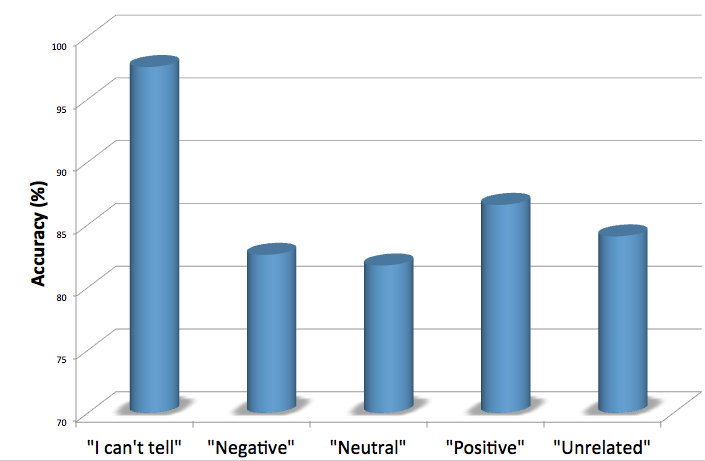
\includegraphics[width=\linewidth]{results/svmSentiment}
  \caption{``Sentiment'' Accuracy}\label{fig:svmSentiment}
\endminipage\hfill
\minipage{0.45\textwidth}
  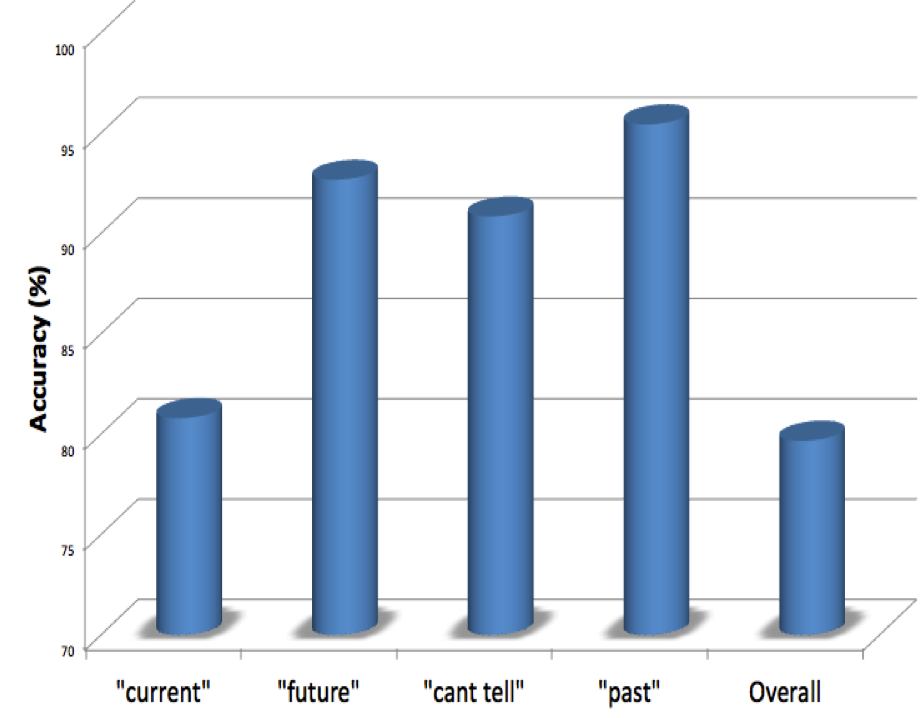
\includegraphics[width=\linewidth]{results/svmWhen}
  \caption{``When'' Accuracy}\label{fig:svmWhen}
\endminipage\hfill
\minipage{0.75\textwidth}%
  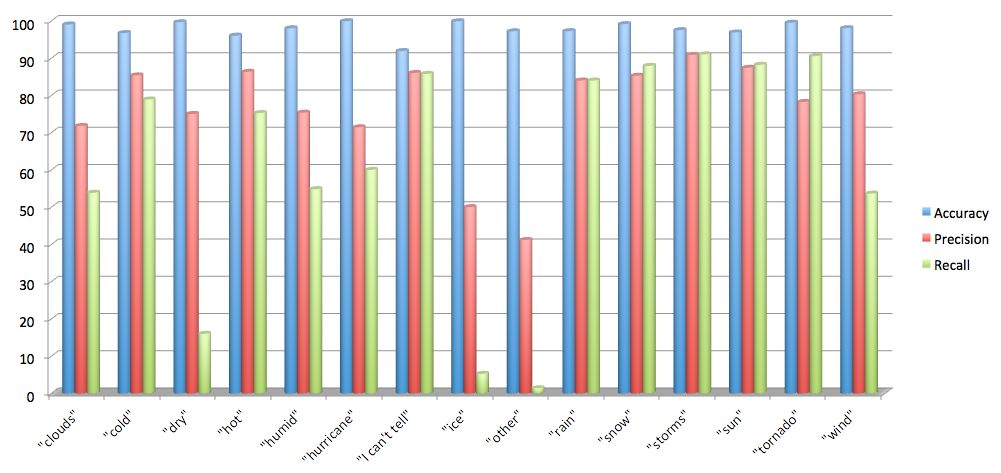
\includegraphics[width=\linewidth]{results/svmKind}
  \caption{Average ``Kind'' Accuracy}\label{fig:svmKind}
\endminipage
\end{figure}
 
We can clearly see from these graphs that accuracies vary a lot by classifier. That may depend very heavily on how many tweets of that category exist in the dataset. For the ``when'' category, it is visible that even though the data is skewed in the direction of the ``current'' label (as the overall accuracy and the ``current'' accuracy are almost the same), it is evident that the other classifiers perform extremely well (high accuracies seen in the ``when'' graph) even though there are few tweets that have those labels. The ``sentiment'' classifier, performs moderately well because of the ambiguities that were mentioned previously. The ``kind'' graph has more detailed precision and recall values telling us the exact combination of true (positives and negatives) and false (positives and negatives) classifications of the validation dataset. A thing to notice here is that the precision values, that tell us the positive predictive value of the relevant tweets is also pretty high for most of the classifiers, but the recall values, which tells us the sensitivity of the classifier, vary heavily across the labels. This could be because our classification is based on a certain number of assumptions, the biggest of them being the use of ``important'' words in classification. The use of these words might make the classifier for some labels less ``sensitive'' and some others more (might classify directly into +1 or -1 based on the class-conditional probabilities).
 
Furthermore, we see the same over-fitting curve for varying the c-values across all the labels, indicating that the separator would have a ``harder'' margin for certain classifiers because they are better separated in n-dimensional space, and ``softer'' margin for some others. This can be seen in the following graph (generated for the ``sentiment'' category):


\begin{figure}[H]
\minipage{0.45\textwidth}%
  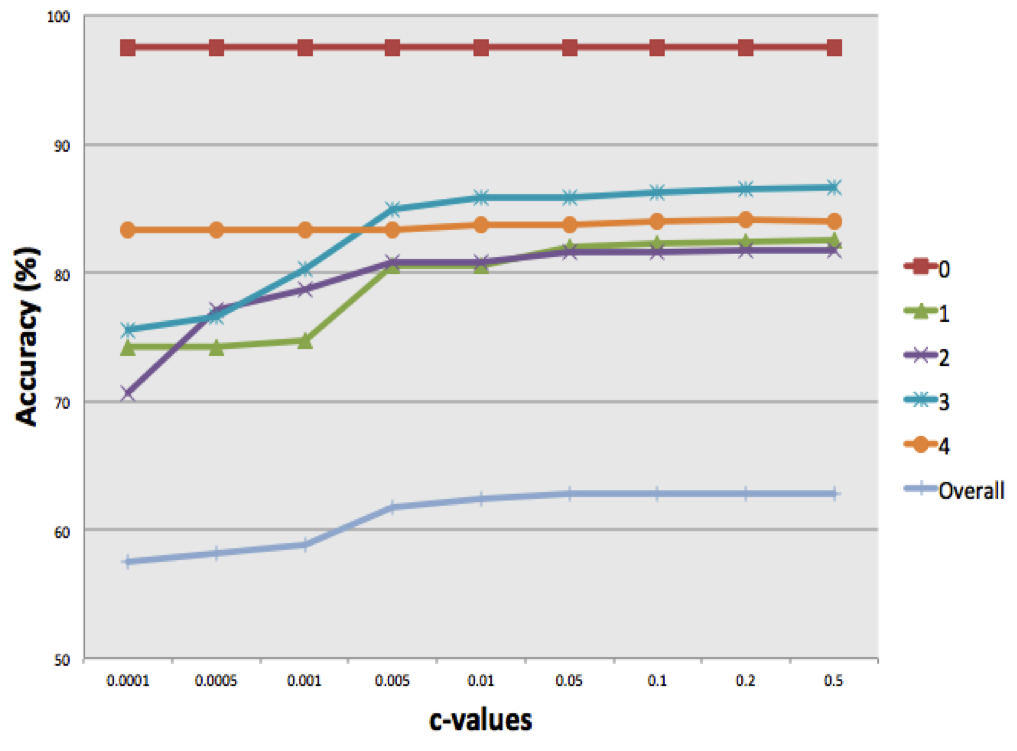
\includegraphics[width=\linewidth]{results/svmCValue}
  \caption{Accuracy vs. C-value}\label{fig:svmCValue}
\endminipage
\end{figure}


\subsubsection{Naive Bayes}
	We observed varying levels of success for different blends of n-grams. The results for all 8 possible groups of unigrams, bigrams, and trigrams can be seen in the table below. Just sticking with the conventional Naive Bayes algorithm (only using unigrams) performed fairly well. However, our intuition has told us that including bigrams and/or trigrams would lead to higher accuracies, because to infer things from sentences one often need to take context of the sentence into consideration, not just each individual word at face-value, and bigrams/trigrams introduce some level of context.

	The accuracies shown below confirm our intuition. Indeed, adding bigrams and/or trigrams into the mix lef to higher accuracies across the board (i.e. for ``Sentiment'', ``When'', and ``Kind''). And unsurprisingly, using bigrams and trigrams on ther own yielded very poor results. This is to be expected, because although certain individual words may occur frequently for certain labels (e.g. the word ``humid'' shows up frequently when the tweet is about humidity), the pairs of words within which they occur might not occur as frequently and thus not have a high class conditional probability. 

	Interestingly, using bigrams and trigrams at the same time produced slightly lower accuracies than using them individually with unigrams, but the difference in accuracy seems too low to come up with an uncontrived justification.
	
%NAIVE BAYES ACCURACY CHART
\begin{figure}[H]
\noindent\makebox[\textwidth][c]{%
\minipage{0.75\textwidth}%
  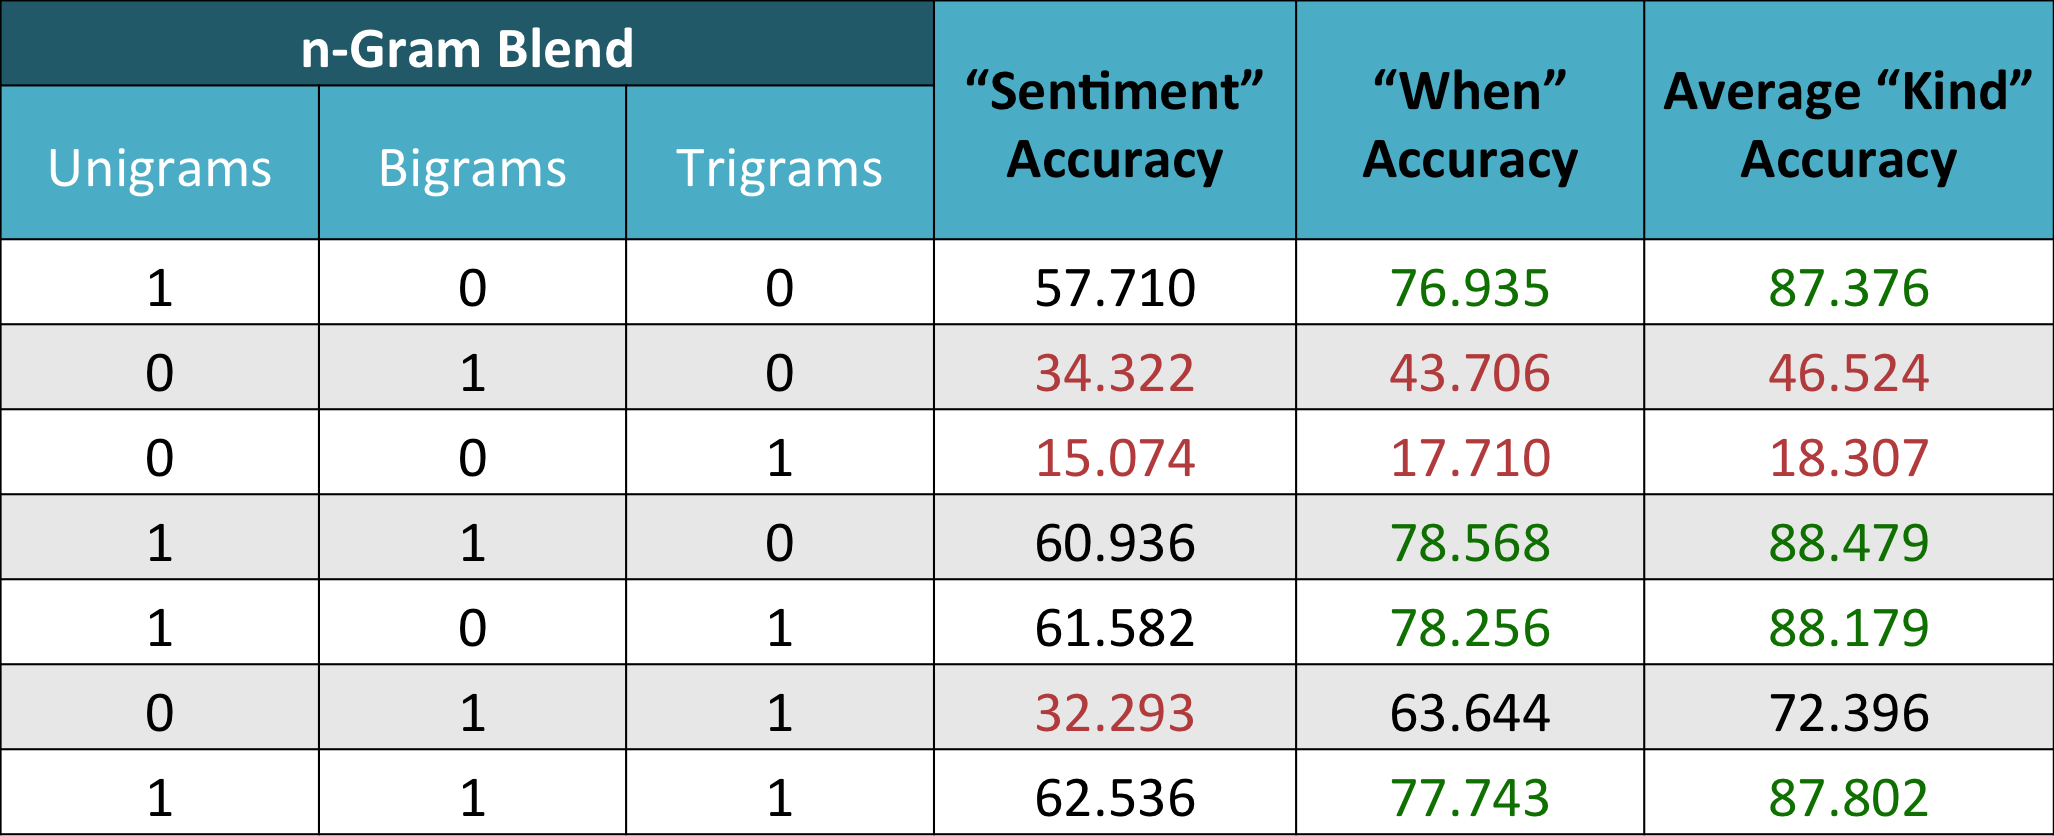
\includegraphics[width=\linewidth]{results/bayes}
  \caption{Accuracy Comparison of n-gram Blends}\label{fig:bayes}
\endminipage}
\end{figure}
